

\section{Введение}
\subsection{Цель работы}
\begin{enumerate}
    \item Проверка принципа эквивалентности масс.
    \item Измерение ускорения свободного падения тел.
    \item Знакомство с методом измерения интервалов времени между импульсами частотомером-хронометром Ч3-32.
    \item Определение погрешности косвенных измерений.
\end{enumerate}
\subsection{Решаемые задачи}
\begin{enumerate}
    \item Вычислить массу каждого шарика.
    \item Зафиксировать время пролета шариков t,мс и вычислить среднее значение времени пролета для каждого шарика.
    \item Вычислить погрешность времени $\Delta$t пролета шариков, используя методы статистической обработки результатов эксперимента.
    \item Вычислить ускорение свободного падения g для каждого шарика.
    \item Определить погрешности измерения $\Delta$g как погрешности косвенных измерений для каждого шарика. Предварительно сделать вывод формулы для определения $\Delta$g.
    \item Проанализировать возможные источники систематических ошибок.
    \item Сделать выводы из данных эксперимента.
\end{enumerate}

\section{Основная часть}

\subsection{Теоретическая часть}

\paragraph{Измерения}

Формула для нахождения среднего арифметического $\overline{U}$:
\begin{equation}
  \overline{t} = \frac{\sum_{i=1}^{n} t_i}{n}
\end{equation}
где $n$ - количество результатов отдельных наблюдений, $t_i$ - результат измерения отдельного наблюдения.

Среднеквадратичное отклонение $\sigma$:
\begin{equation}
   \sigma \approx \sqrt{\frac{1}{n-1} \sum_{i = 1}^{n} (t_i -\overline{t}^2)}
\end{equation}

Погрешность среднеарифметического результата наблюдений
\begin{equation}
   s_{\overline{t}}=\frac{\sigma}{\sqrt{n}}
\end{equation}

Как известно, уравнение движения при свободном падении имеет вид:
\begin{equation}
  h = v_0 t + \frac{gt^2}{2}
\end{equation}

Функция $g$ зависит от трех переменных: $h, \ t, \ v_0$:
\begin{equation}
  g = \frac{2(h - v_0 t)}{t^2}
\end{equation}
Погрешность измерения величин $h, \  v_0$ определяется погрешностью измерительных приборов $\omega_{h}, \ \omega_{v_0}$; погрешность прямо измеряемой величины $t$  является случайными величинами, это означает, что погрешность для $t$ определяется погрешностью среднеарифметического результата наблюдений  $s_{\overline{t}}$. Следовательно формула для нахождения косвенной погрешности $\Delta g$ будет выглядеть следующим образом:

\begin{equation}
  \Delta g \approx \sqrt{\frac{1}{9} \left( \frac{\partial g}{\partial h} \right)^2 \omega_h^2 +\frac{1}{9} \left( \frac{\partial g}{\partial v_0} \right)^2 \omega_{v_0}^2 + \left( \frac{\partial g}{\partial t} \right)^2 s_{\overline{t}}^2}
\end{equation}

Найдем частные производные: $\frac{\partial g}{\partial h} = \frac{2}{t^2}$;
$\frac{\partial g}{\partial v_0} = -\frac{2}{t}$;
$\frac{\partial g}{\partial t} = \frac{2(v_0 t - 2h)}{t^3}$.


Итоговое уравнения для $\Delta g$:
\begin{equation}
  \Delta g \approx \sqrt{\frac{1}{9} \left( \frac{2}{t^2} \right)^2 \omega_h^2 +\frac{1}{9} \left( -\frac{2}{t} \right)^2 \omega_{v_0}^2 + \left( \frac{2(v_0 t - 2h)}{t^3} \right)^2 s_{\overline{t}}^2}
\end{equation}

\subsection{Эксперимент}
Схема установки приведена на рис. 1. Луч от квантового генератора ЛГ направляется на призму полного внутреннего отражения П$_1$, от нее на призму П$_2$, а затем на фотодиод ФД. При отодвигании заслонки З шарик, находящийся в трубке Т, падает в лузу Л и пересекает два световых луча, расстояние между которыми равно h. Когда шарик пересекает верхний луч, фотодиод ФД вырабатывает импульс, который усилившись в усилителе, подается на вход частотомера Ч3-32 и запускает его. При пересечении шариком нижнего луча импульс от фотодиода останавливает счет частотомера. Интервал времени между двумя импульсами, регистрируемый частотомером, равен времени пролета t шарика от верхнего луча до нижнего. Усилитель питается от источника УПУ-1У4. 

Были заданы следующие значения для эксперимента:
\begin{enumerate}
    \item $h = (0.272 \pm 0.001)$ м $=> \omega_h = 0.001$ м; 
    \item $v_0 = (1.050 \pm 0.005) \ \text{м} / \text{с}$ $=> \omega_{v_{0}} = 0.005 \ \text{м} / \text{с}$;
\end{enumerate}

\begin{figure}[ht!]
\centering
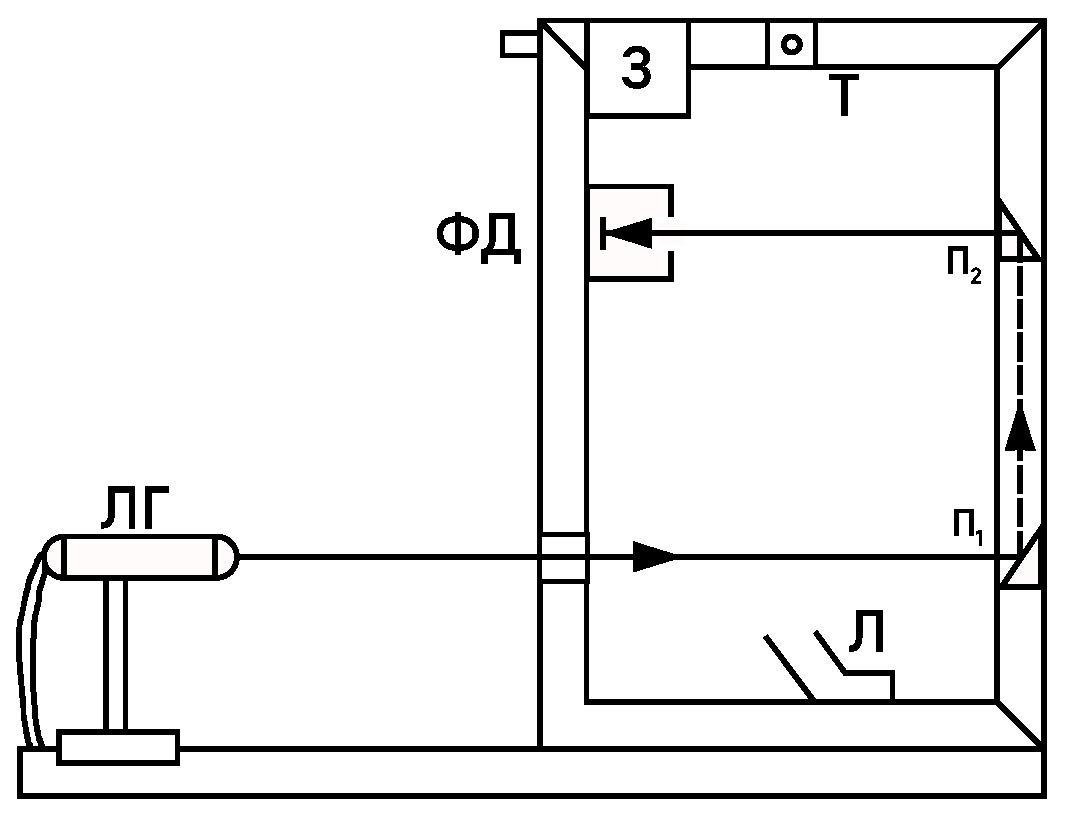
\includegraphics[width=0.8\textwidth]{схема_с_лазером.eps}
\caption{Схема установки}
\label{fig:sketch}
\end{figure}

\subsection{Обработка данных и обсуждение результатов}

\subsubsection{Исходный код}
Для написания программы, вычисляющей все требуемые данные, используется язык C++; среда разработки - Visual Studio.

Программа обрабатывает значения для разных шариков по выведенным формулам: нахождение среднего арифметического, нахождение погрешности среднеарифметического результата наблюдений, нахождение косвенной погрешности, нахождение масс шариков, нахождение ускорения свободного падения.

Все выполненные вычисления заносятся в файлы с расширением .csv в соответствующих папках.

\begin{lstlisting}[label=listing1, caption=Функция для нахождения $\Delta g$]
std::vector<double> delta_g(std::vector<double>& avarage, std::vector<double>& delta_t)
{
	std::vector<double> arr(6, 0);
	for (int i = 0; i < 6; i++)
	{
		double t_i = avarage[i] / 1000;
		double tt = std::pow(t_i, 4);
		double te = tt;
		double c_h = 4 / (9 * std::pow(t_i, 4));
		double c_v_0 = 4 / (9 * std::pow(t_i, 2));
		double c_t = ((2 * V_0 * t_i - 4 * H) / (t_i * t_i * t_i)) * ((2 * V_0 * t_i - 4 * H) / (t_i * t_i * t_i));
		arr[i] = sqrt(c_h * omega_h * omega_h + c_v_0 * omega_v_0 * omega_v_0 + (delta_t[i] * delta_t[i] * c_t / 1000000)) / sqrt(30);
	}

	return arr;
}
\end{lstlisting}

\begin{lstlisting}[label=listing2, caption=Функция для нахождения $\Delta t$]
std::vector<double> delta_T(const std::vector<std::vector<double>>& data, std::vector<double>& avarage)
{
	std::vector<double> delta_t(6, 0);
	for (int i = 1; i < 7; ++i)
	{
		double sum = 0.0;
		for (int j = 0; j < 29; ++j)
		{
			double d = (data[j][i] - avarage[i - 1]);
			sum += d * d;
		}
		delta_t[i - 1] = sqrt((sum) / (data.size()));
		delta_t[i - 1] /= sqrt(30);
	}

	return delta_t;
}
\end{lstlisting}
\newpage
\subsubsection{Таблицы}


\begin{center}
\begin{table}[h!]
\centering
\caption{Результаты измерения времени падения шарика от верхнего луча до нижнего}
\label{tabl:2}
\begin{tabular}{|c|c|c|c|c|c|c|}
\hline
№ п.п.& Алюминий & Латунь & Сталь & Дерево & Плексиглас & Свинец \\
\hline
{}&t, мс&t, мс&t, мс&t, мс&t, мс&t, мс\\
\hline
1&153.963&153.692&152.337&154.324&153.326&153.391 \\
2&153.612&152.895&153.777&154.011&154.178&153.225 \\
3&153.178&153.065&152.616&154.378&153.245&153.900 \\
4&152.978&152.845&152.725&155.019&153.199&153.449 \\
5&153.161&153.401&152.687&154.112&153.737&152.773 \\
6&152.647&152.962&154.121&154.393&154.022&153.258 \\
7&153.265&152.633&152.557&154.121&153.335&152.291 \\
8&153.572&152.806&153.033&154.101&154.341&154.345 \\
9&153.623&152.819&153.153&154.989&154.471&152.916 \\
10&152.611&152.751&152.401&154.949&153.404&152.599 \\
11&153.421&152.841&152.678&154.606&153.550&153.426 \\
12&154.882&152.773&152.277&154.464&153.451&153.675 \\
13&152.989&152.850&152.409&155.113&153.386&153.938 \\
14&152.824&152.751&152.603&154.778&153.501&153.684 \\
15&152.783&152.702&152.853&153.991&153.400&153.276 \\
16&152.746&152.724&152.832&154.140&153.963&152.910 \\
17&152.842&152.884&153.355&154.445&153.233&154.140 \\
18&152.891&152.496&153.667&154.196&154.007&153.345 \\
19&153.835&153.117&152.983&154.064&153.637&153.159 \\
20&154.131&152.747&152.785&154.473&153.864&153.651 \\
21&152.993&152.873&152.737&154.428&153.449&152.719 \\
22&153.223&153.818&152.678&153.973&154.632&153.106 \\
23&152.919&152.840&152.504&154.395&153.454&152.807 \\
24&153.328&152.903&153.240&154.187&153.939&153.140 \\
25&152.746&152.838&152.891&154.339&153.230&153.009 \\
26&152.994&153.153&153.839&154.208&153.881&153.000 \\
27&153.937&153.566&152.704&153.774&153.907&153.333 \\
28&153.441&153.451&152.919&154.772&153.796&153.048 \\
29&153.144&152.873&153.478&154.012&153.453&153.144 \\
30&153.325&152.093&152.752&154.277&153.361&153.804 \\
\hline
$\overline{t}$&153.247 &152.933 &152.918 & 154.378&153.68&153.286 \\ 
\hline
\end{tabular}
\end{table}
\end{center}

\begin{center}
\begin{table}[h!]
\centering
\caption{Таблица веществ}
\label{tabl:1}
\begin{tabular}{|c|c|c|c|}
\hline
\begin{minipage}{1cm}
    №№ п/п 
\end{minipage} &
    
\begin{minipage}{5cm}
    Вещество
\end{minipage} &
\begin{minipage}{5cm}
    Плотность ($10^3 \frac{\text{кг}}{\text{м}^{3}}$)
\end{minipage} &
 Масса (10$^{-6}$)
\\
\hline
1 & дерево (береза) & 0.7 & 0.37\\
2 & плексиглас & 1.18 & 0.62\\
3 & дуралюминий & 2.79 & 1.46\\
4 & сталь & 7.9 & 4.14\\
5 & латунь & 8.5 & 4.45\\
6 & свинец & 11.34 & 5.94\\
\hline
\end{tabular}
\end{table}
\end{center}

\begin{center}
\begin{table}[h!]
\centering
\caption{Погрешность времени пролета шариков}
\label{tabl:3}
\begin{tabular}{|c|c|c|}
\hline
\begin{minipage}{1cm}
    №№ п/п
\end{minipage}
 & Вещество & $\Delta$t, мс \\
\hline
1 & Алюминий & 0.091\\
2 & Латунь & 0.064\\
3 & Сталь & 0.086\\
4 & Дерево & 0.062\\
5 & Плексиглас & 0.071\\
6 & Свинец & 0.085\\
\hline
\end{tabular}
\end{table}
\end{center}

\begin{center}
\begin{table}[h!]
\centering
\caption{Ускорение свободного падения g для каждого шарика}
\label{tabl:3}
\begin{tabular}{|c|c|c|}
\hline
\begin{minipage}{1cm}
    №№ п/п
\end{minipage}
 & Вещество & g, $\frac{\text{м}}{\text{c}^2}$ \\
\hline
1 & Алюминий & 9.460\\
2 & Латунь & 9.527\\
3 & Сталь & 9.531\\
4 & Дерево & 9.223\\
5 & Плексиглас & 9.369\\
6 & Свинец & 9.452\\
\hline
\end{tabular}
\end{table}
\end{center}

\begin{center}
\begin{table}[h!]
\centering
\caption{Погрешности косвенных измерений для
каждого шарика}
\label{tabl:5}
\begin{tabular}{|c|c|c|}
\hline
\begin{minipage}{1cm}
    №№ п/п
\end{minipage}
 & Вещество & $\Delta$g, $\frac{\text{м}}{\text{c}^2}$ \\
\hline
1 & Алюминий & 0.041\\
2 & Латунь & 0.038\\
3 & Сталь & 0.040\\
4 & Дерево & 0.038\\
5 & Плексиглас & 0.038\\
6 & Свинец & 0.040\\
\hline
\end{tabular}
\end{table}
\end{center}
Систематические ошибки — это ошибки, которые приводят к отклонению результатов измерений в одном направлении (либо завышают, либо занижают). Их сложнее обнаружить, чем случайные ошибки.

Инструментальная погрешность всегда неизвестна и зависит от внешних условий (температуры, давления, влажности и т. д.). Поэтому любой измерительный прибор, изготовленный и проверенный на заводе-изготовителе, снабжается паспортом, где в числе других
его характеристик указывается предел допускаемой погрешности. Инструментальные погрешности отражают суммарное действие разнообразных факторов, приводящих к возникновению как систематических, так и случайных погрешностей. В нашем случае усилитель, частотомер или фотодиоды могут вносить небольшую, но систематическую задержку в измерение времени. Также нужно не забывать, что в установке присутствует неидеальная призма, из-за этого может незначительно изменять траекторию луча или вносить задержку.

Значения погрешности $\Delta$g для разных материалов лежат в относительно узком диапазоне (от 0.038 до 0.041 м/с²). Это говорит о том, что основные источники погрешностей, вероятно, связаны не с конкретным материалом шарика, а с общими факторами, такими как точность измерительных приборов, сопротивление воздуха или ошибки наблюдателя.

Все измеренные значения g систематически занижены по сравнению со значением 9.81 м/с², это указывает на наличие систематических ошибок.

\section{Вывод}
Эксперимент показывает важность учета различных факторов, влияющих на точность измерений. Для повышения точности результатов необходимо тщательно анализировать и минимизировать влияние систематических ошибок.
% Список литературы
% Для отчёта он не обязателен
\begin{thebibliography}{9}

%ссылка на репозиторий с исходныим кодом отчета и всех расчетных программ обязательна 
\bibitem{repo}
\url{https://github.com/st117210/Workshop1.git}  

\end{thebibliography}
\clearpage
\appendix